\documentclass[UTF8]{ctexart}
\usepackage{CJKutf8}
\usepackage{graphicx}
\usepackage{amsmath}
\usepackage{diagbox}
\usepackage{hyperref}
\usepackage{xcolor}
\usepackage[linesnumbered,boxed,ruled,commentsnumbered]{algorithm2e}
\usepackage{cite}

  \author{黄晃\ 数院 1701210098 }
  \title{homework-sto}
\begin{document}

  \maketitle
  \section{问题}
  原问题为
  \begin{equation}\label{p:1}
    \begin{split}
       min\  &  \frac{1}{n}f_i(w)+\lambda\|w\|_1 \\
    \end{split}
  \end{equation}
  where $f_i(w)=log(1+exp(-y^iw^Tx^i)and lambda>0$
  \paragraph{}
  为了使用stochastic optimization,可以将问题改写成
    \begin{equation}\label{p:2}
    \begin{split}
       min\  &  \frac{1}{n}f_i(w)\\
    \end{split}
  \end{equation}
  where $f_i(w)=log(1+exp(-y^iw^Tx^i)+\lambda\|w\|_1$
  \subsection{数据集}
    使用要求的两个数据集:MINIST和Coverttype.
    \paragraph{MINIST}
    一共70000个样本,其中每个$x^i$是28*28的灰度矩阵向量化的结果,而$y^i$是该幅图片对应的label
    \paragraph{Covertype}
    一共581012个样本,其中每个$x^i$是54维向量
    \paragraph{数据归一化}
    对于$X=[x_1,x_2,\cdots,x_N]=[a_1,a_2,\cdots,a_p]^T$,我们对其进行行归一化,即取$\hat{X}=[\hat{a_1},\hat{a_2},\cdots,\hat{a_p}]^T$,其中$\hat{a_i}=a_i/max(a_i)$
    \subsection{算法}
  一共实现了要求的两个算法:SAG和SVRG以及附加任务:使用BB步长的SG方法
  \subsubsection{SAG}

\begin{algorithm}

    \SetAlgoNoLine % 不要算法中的竖线
    \SetKwInOut{Input}{\textbf{输入}}\SetKwInOut{Output}{\textbf{输出}} % 替换关键词

    \Input{
        \\
        The observed user-item pair set $S$\;\\
        The feature matrix of items $F$\;\\
        The content features entities $A := \{A^u,A^v\}$\;\\}
    \Output{
        \\
        $\Theta \  := \{Y^u,Y^v\}$\;\\
        $W := \{W^u,W^v\}$\;\\}
    \BlankLine

    initialize the model parameter $\Theta$ and $W$ with uniform $\left(-\sqrt{6}/{k},\sqrt{6}/{k}\right)$\; % 分号 \; 区分一行结束
    standarized $\Theta$\;
    Initialize the popularity of categories $\rho$ randomly\;
    \Repeat
        {\text{convergence}}
        {Draw a triple $\left(m,i,j\right)$ with 算法\ref{al2}\;
            \For {each latent vector $\theta \in \Theta$}{
                $\theta \leftarrow \theta - \eta\frac{\partial L}{\partial \theta}$
            }
            \For {each $W^e \in W$}{
                Update $W^e$ with the rule defined in Eq.\ref{equ:W}\;
            }
        }
    \caption{Learning paramters for BPR\label{al3}}
\end{algorithm}

  $$w_{k+1}=w_k-\alpha_k(\frac{1}{n}(\nabla f_{s_k}(w_k)-g_{k+1}^{s_k})+\frac{1}{n}\sum_{i=1}^{N}g_{k-1}^i)$$
  其中
  \begin{equation*}
    g_k^i= \left\{
    \begin{array}{cc}
      \nabla f_{i}(w_k) &if\ i=s_k\\
      g_{k+1}^{s_k} & else
    \end{array}
    \right.
  \end{equation*}
  所以需要存储每个$f_i$随着随机量$s_K$最近一次被计算时得到的值作为$g_k^i$.此外,为了启动算法,在第一次迭代开始前,对每个$f_i$计算一次相应的次梯度
  \subsubsection{SVRG}
  如课件所示,每求一次完整的函数f的梯度,进行m次随机梯度的迭代,然后将结果的平均作为外部循环的结果.每次内循环的下降方向选择为
  $$
  v_k=\nabla f_{s_k}(w_k)-\nabla f_{s_k}(y)+\nabla f(w_i)
$$
其中$w_i$为外循环第i步的值
\subsubsection{SG-BB(Extra-credit)}
  $$
  w_k+1= w_k + \alpha_k \nabla f_{s_k}(w_k)
$$
其中
\begin{equation*}
\begin{split}
\alpha_k = \frac{(s^{k-1})^Ty^{k-1}}{(y^{k-1})^Ty^{k-1}} \\
s^{k-1}=w^k-w^{k-1},\\
 y^{k-1}=g^k-g^{k-1}
\end{split}
\end{equation*}
其中$g^k=\nabla f_{s_k}(w_k)$为第k次计算的随机梯度,而不是完整函数的梯度
\subsection{计算细节}
在计算函数值以及梯度时会遇到如下两类问题
\begin{itemize}
  \item 计算$\frac{e^x}{1+e^x}$时$e^x=inf$
  \item 计算$log(1+e^x)$时$e^x=inf$
\end{itemize}
我们将其处理成$\frac{e^x}{1+e^x}=1,log(1+e^x)=x$
\section{计算结果}

对$\lambda=10,1,0.1,0.001,\frac{1}{n}$进行了实验
\paragraph{参数}
SVRG中$m=\frac{n}{10}$,SVRG以及SAG中$\alpha=0.01$,SVRG一共进行了20次迭代,SAG进行了n次迭代,sgBB进行了2n次迭代.
\paragraph{误差定义}
参考文献定义Testing Error$R(w)=\sum_{i=1}^{n}log(1+exp(-b^iw^Ta^i))$
\paragraph{结果取样}
由于R(w)的计算量太大,在展示结果时,我们只等距的选取了20个点的值来作图
\paragraph{x轴}
仿照参考文献,做了三类图,其x轴分别为迭代次数,求导次数,时间.在这里求导次数定义为单个$f_i$的求导次数.所以SVRG一次迭代求导次数了增加n+m次.
\paragraph{图注}
在每一组图的图注位置,在相应算法后记录最后时刻的R(w)

\subsection{MINIST}
其中最后两幅图与其他略有区别:\ref{fig:1-n-c} 是去掉初始点后,SAG与SVRG的比较;\ref{fig:1-n-sag}是去掉初始点后SAG的R(w).以上两幅图的单独列出是为了排除掉初始点,让函数值的变化看的更清晰(初始点值太大产生比例尺的干扰)
\begin{figure}[htbp]
\centering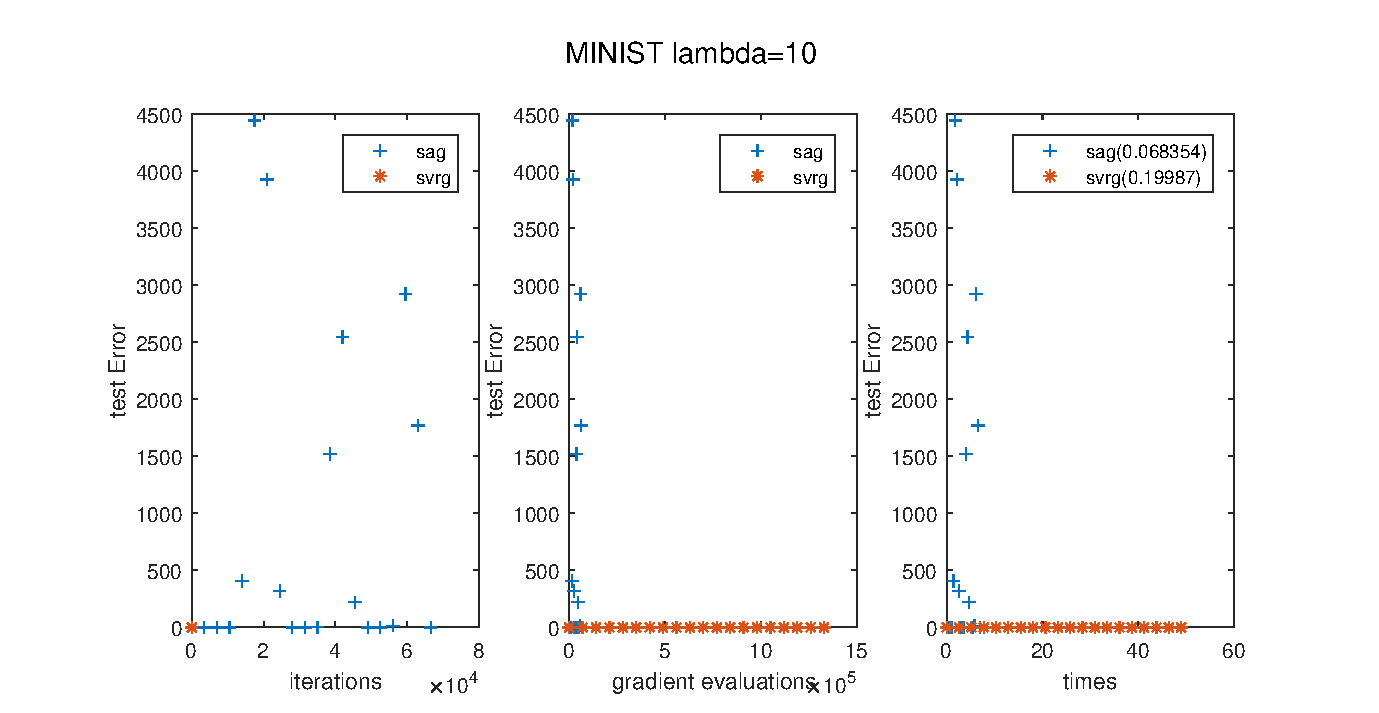
\includegraphics[width=5in]{1-10-a.eps}
\label{fig:1-10-a}
\end{figure}
\begin{figure}[htbp]
\centering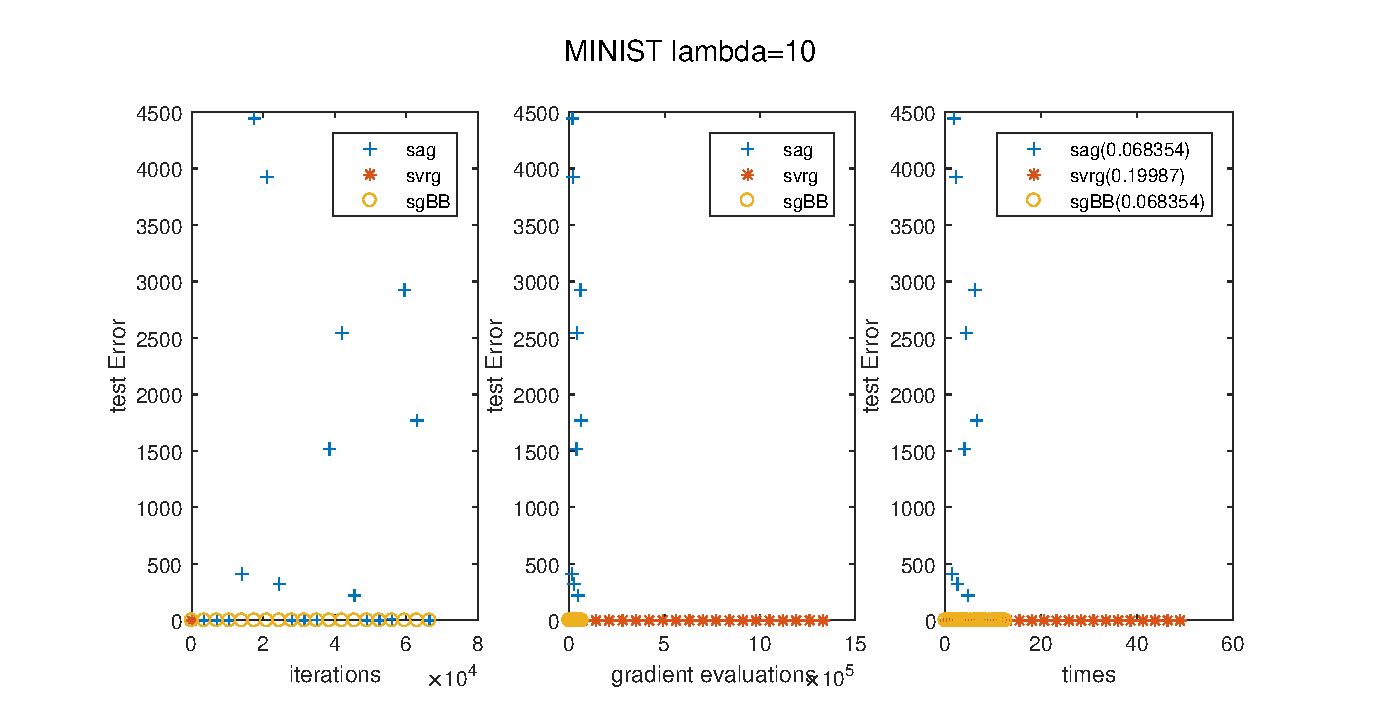
\includegraphics[width=5in]{1-10-b.eps}
\label{fig:1-10-b}
\end{figure}

\begin{figure}[htbp]
\centering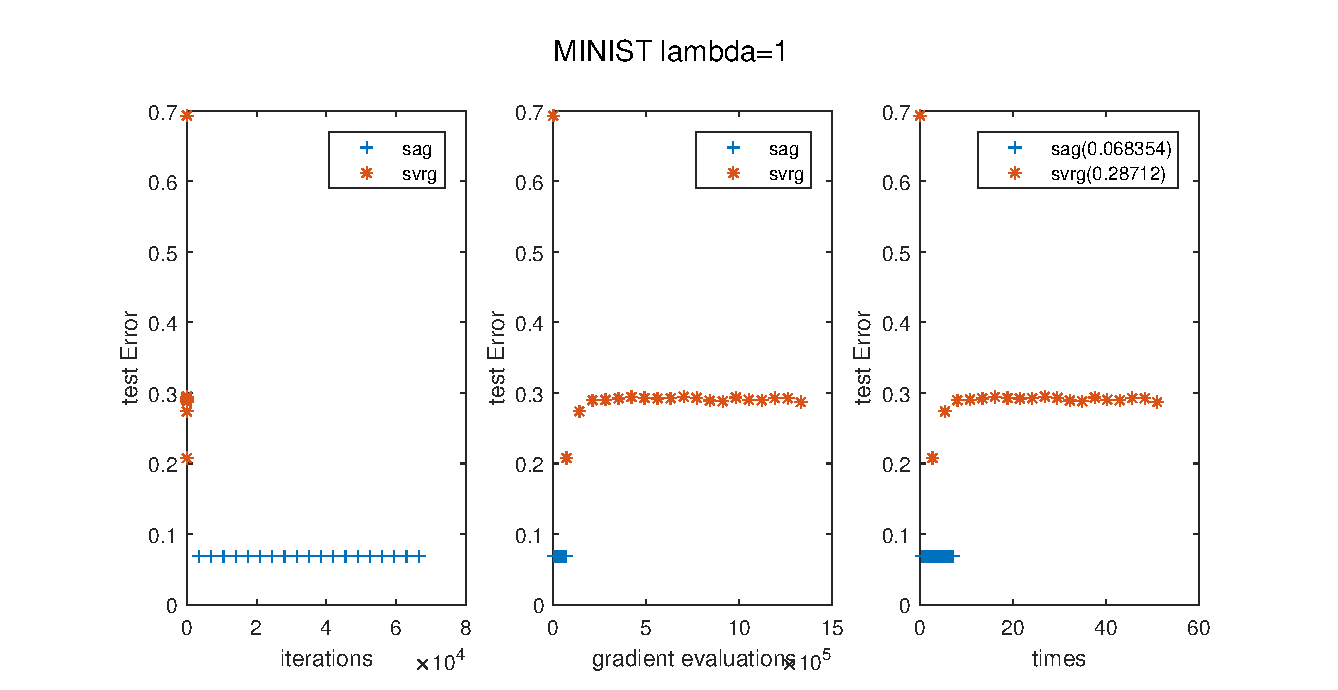
\includegraphics[width=5in]{1-1-a.eps}
\label{fig:1-1-a}
\end{figure}

\begin{figure}[htbp]
\centering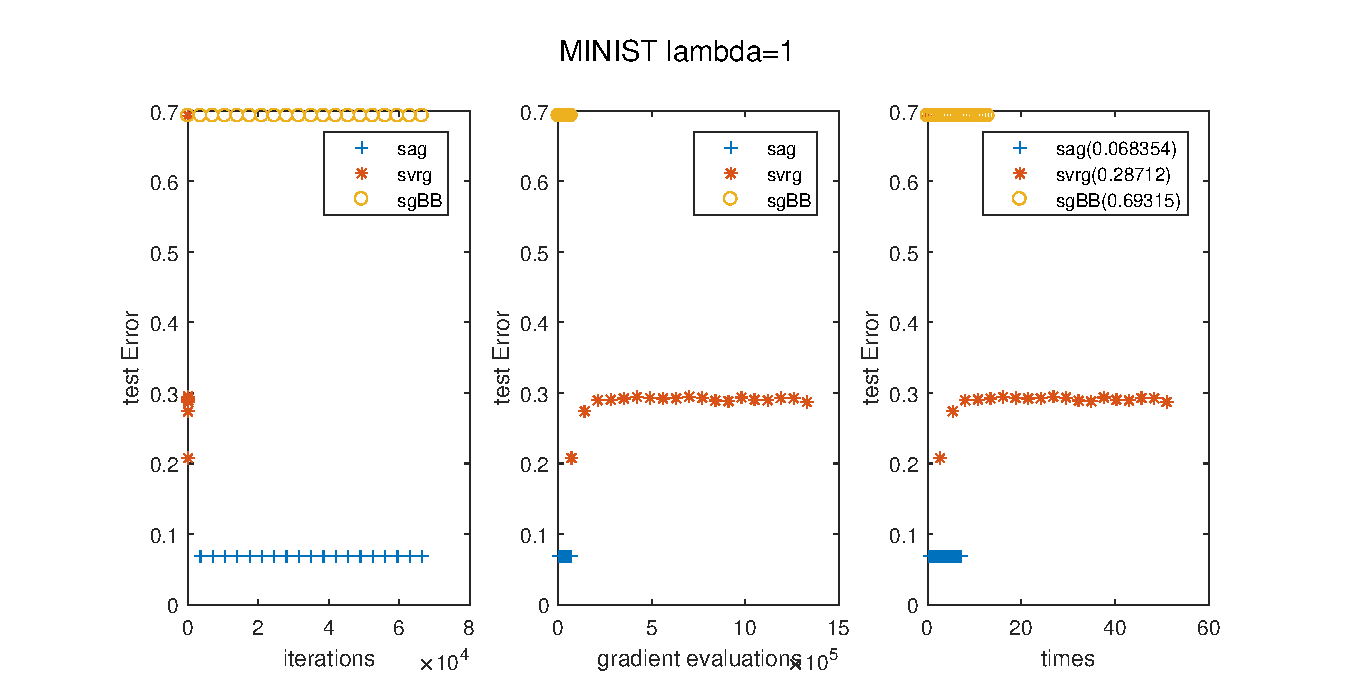
\includegraphics[width=5in]{1-1-b.eps}
\label{fig:1-1-b}
\end{figure}

\begin{figure}[htbp]
\centering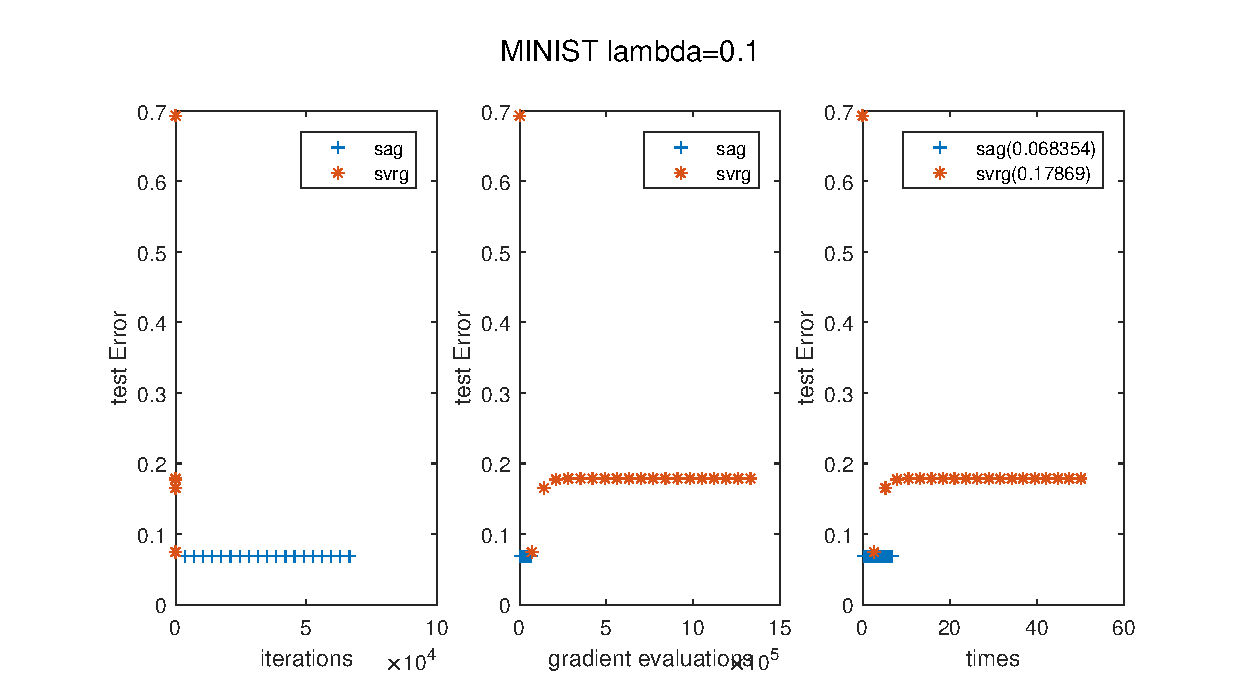
\includegraphics[width=5in]{1-01-a.eps}
\label{fig:1-0.1-a}
\end{figure}

\begin{figure}[htbp]
\centering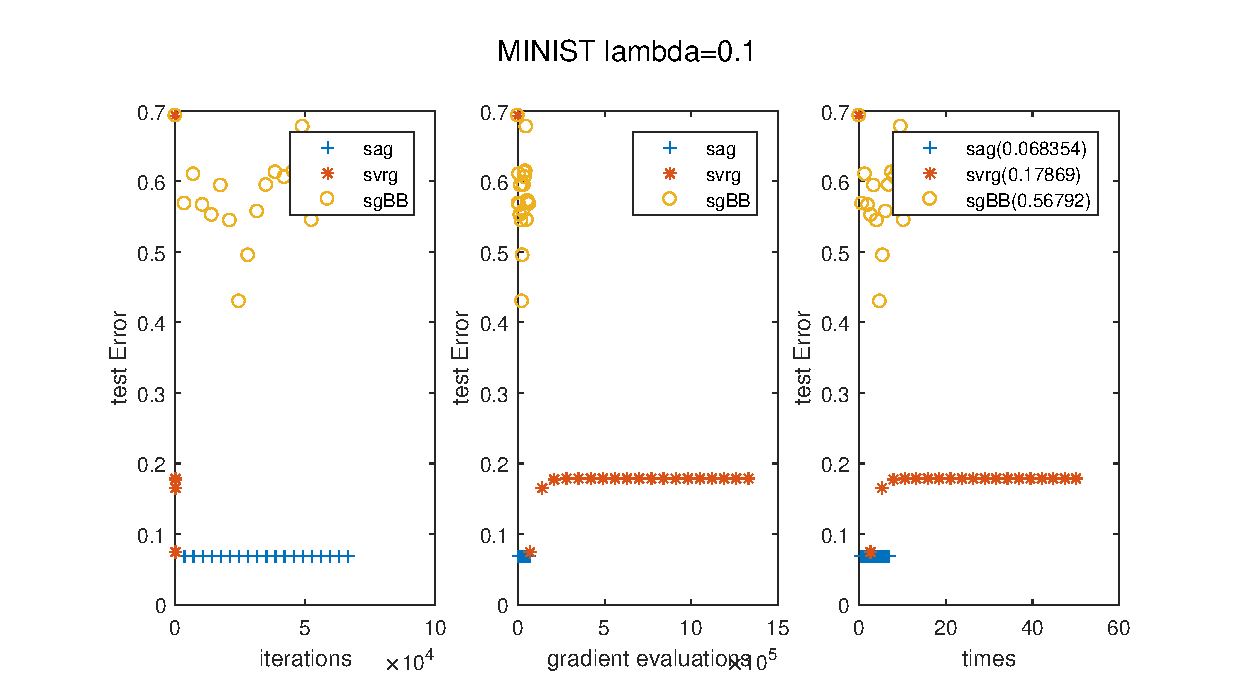
\includegraphics[width=5in]{1-01-b.eps}
\label{fig:1-0.1-b}
\end{figure}
\begin{figure}[htbp]
\centering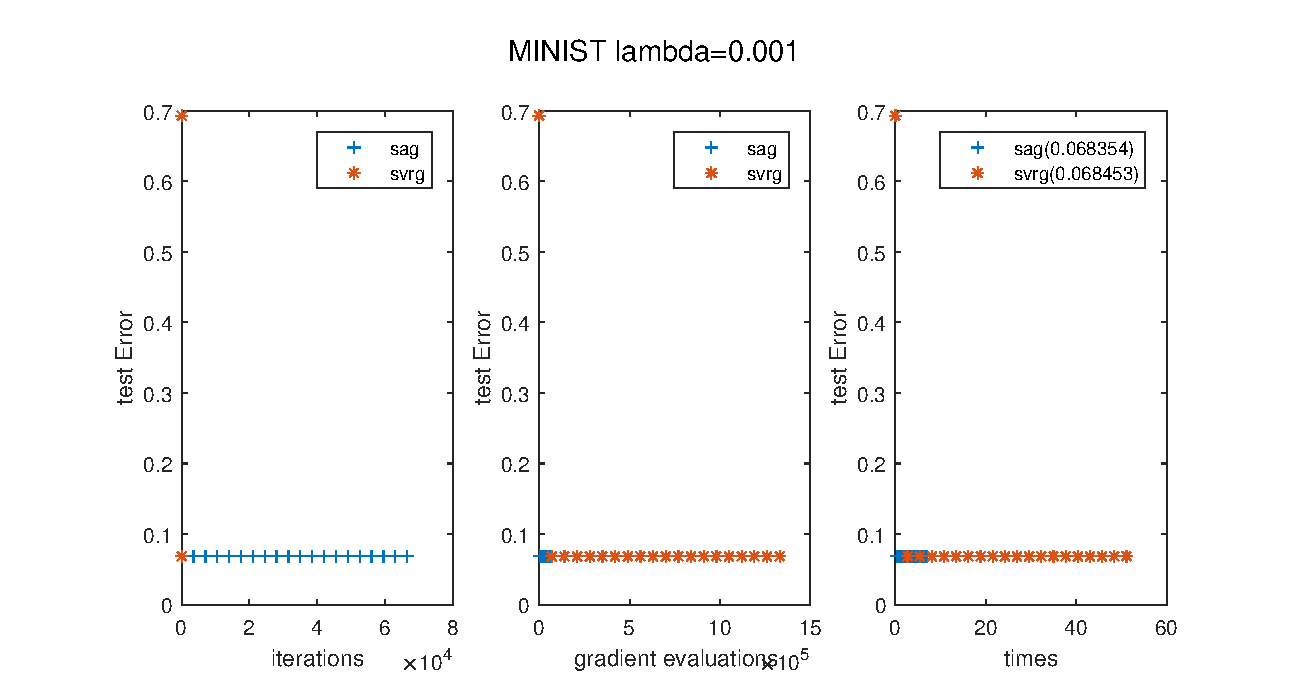
\includegraphics[width=5in]{1-0001-a.eps}
\label{fig:1-0.001-a}
\end{figure}
\begin{figure}[htbp]
\centering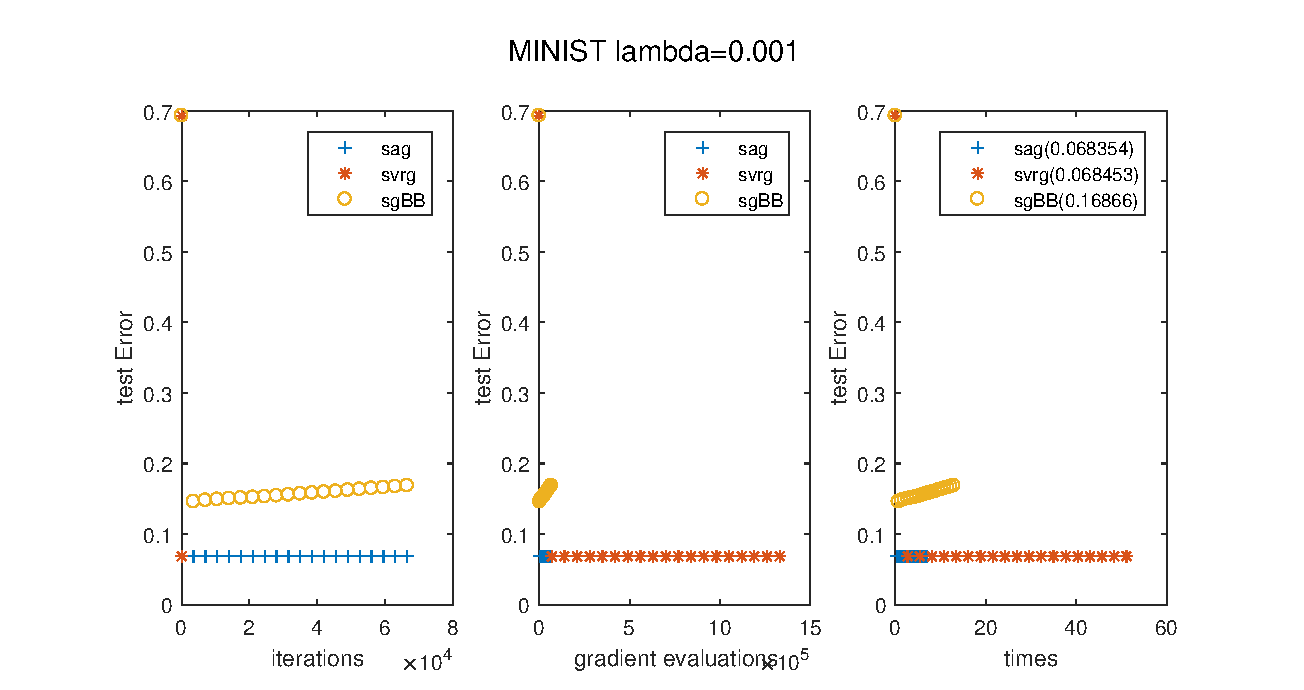
\includegraphics[width=5in]{1-0001-b.eps}
\label{fig:1-0.001-b}
\end{figure}
\begin{figure}[htbp]
\centering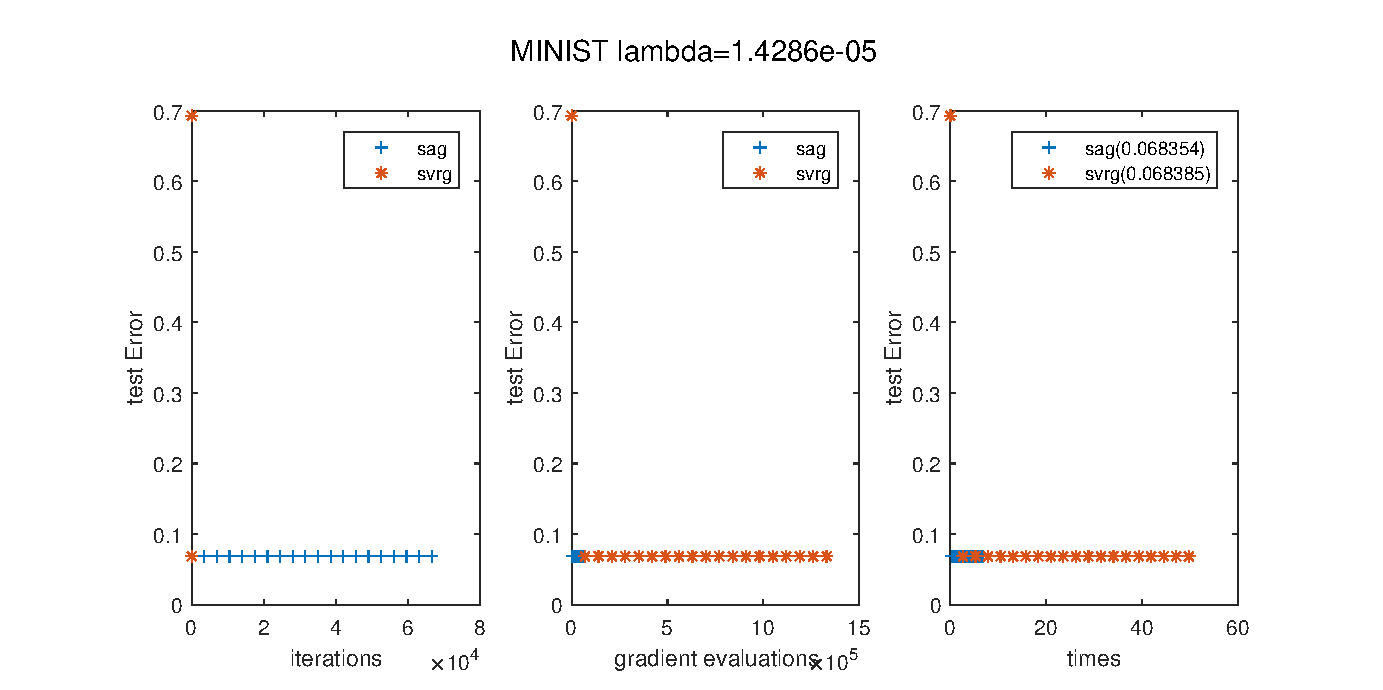
\includegraphics[width=5in]{1-n-a.eps}
\label{fig:1-n-a}
\end{figure}
\begin{figure}[htbp]
\centering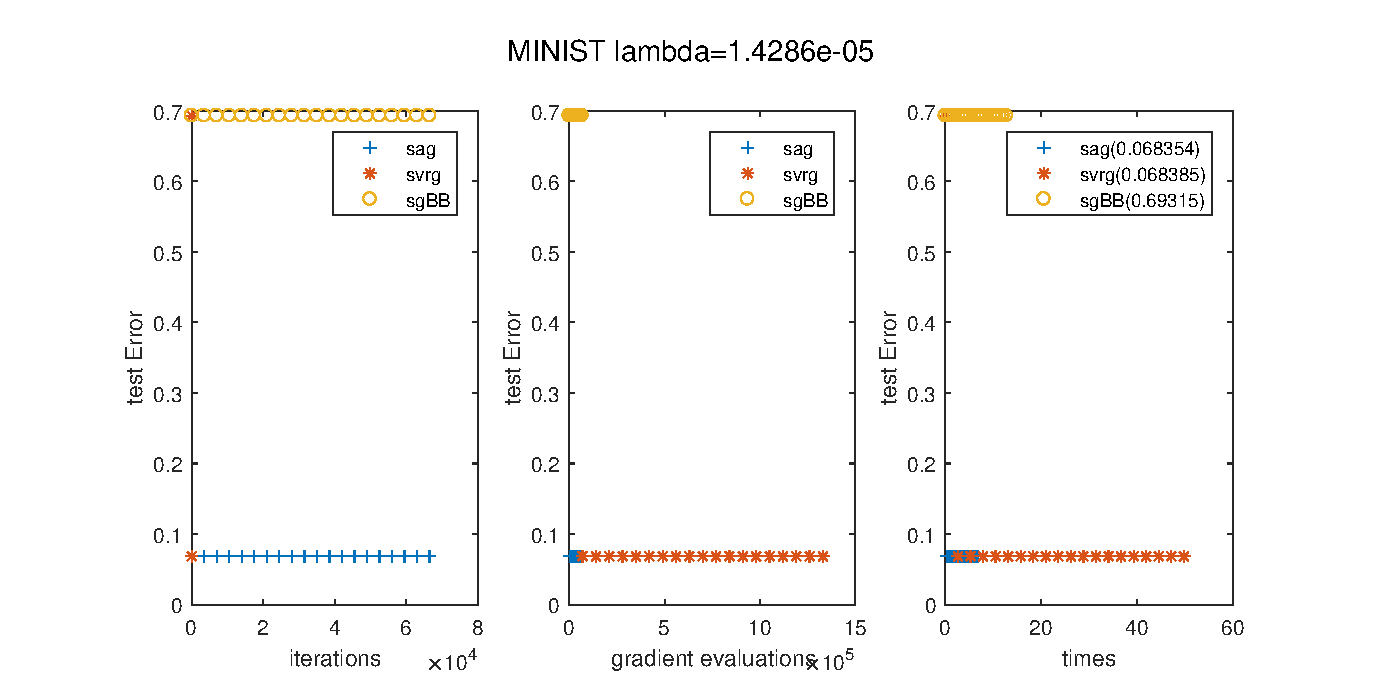
\includegraphics[width=5in]{1-n-b.eps}
\label{fig:1-n-b}
\end{figure}

\begin{figure}[htbp]
\centering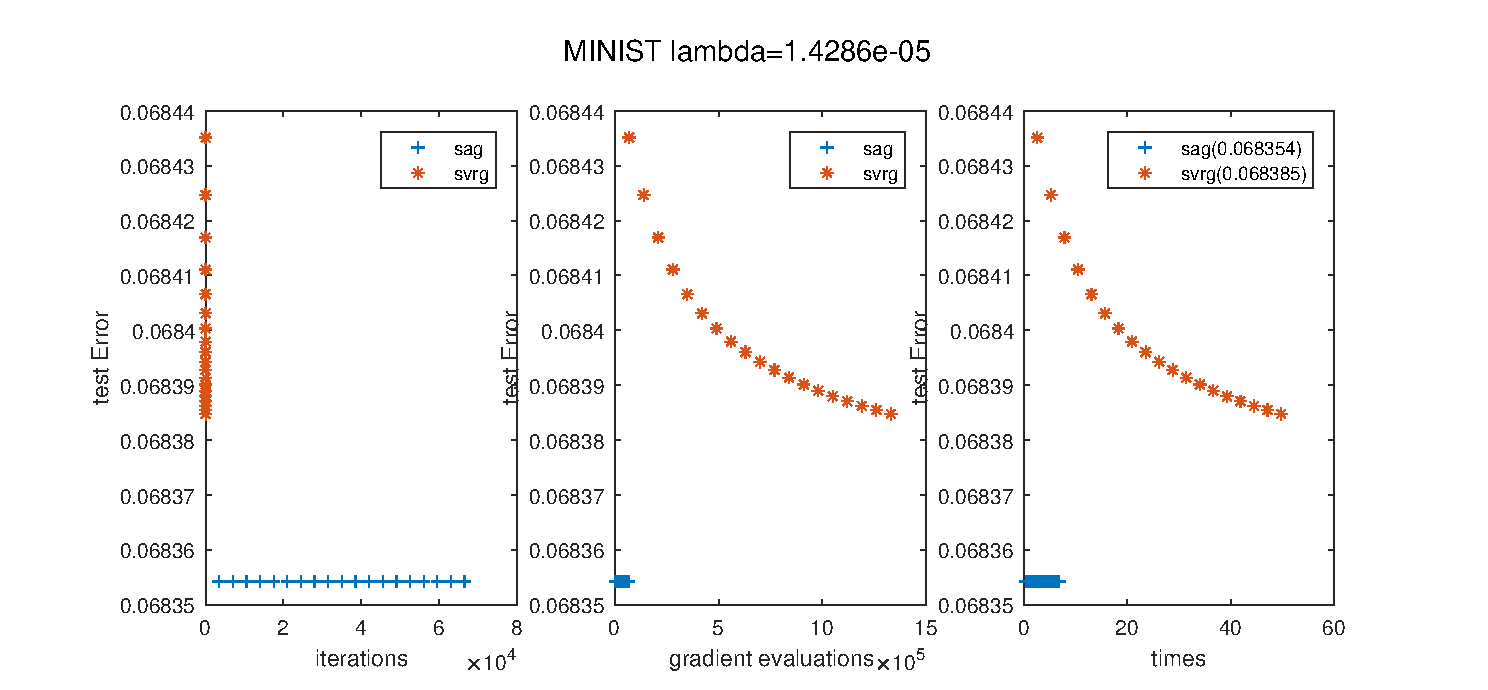
\includegraphics[width=5in]{1-n-c.eps}
\caption{}\label{fig:1-n-c}
\end{figure}

\begin{figure}[htbp]
\centering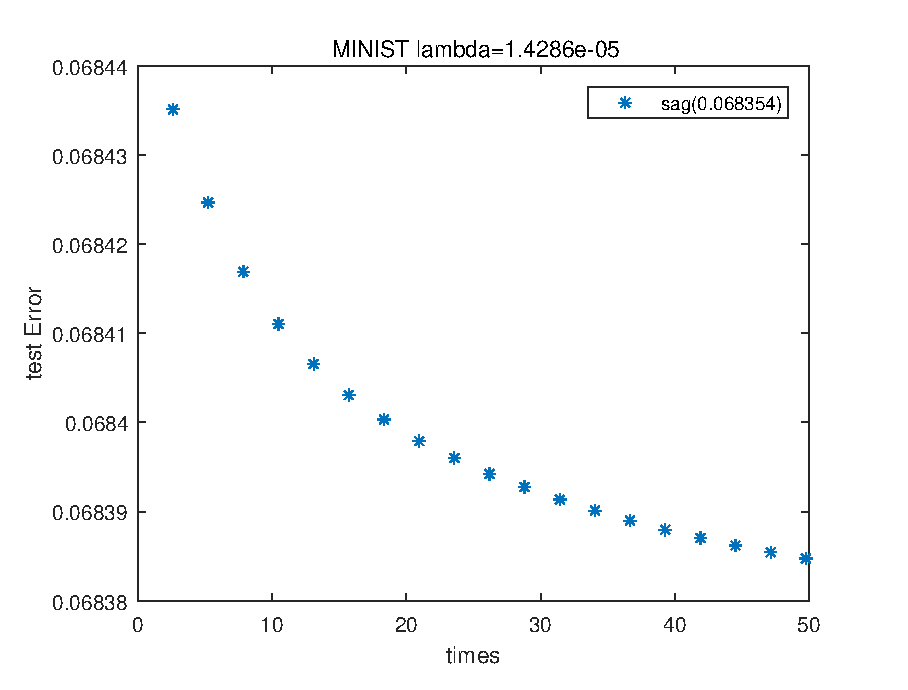
\includegraphics[width=5in]{1-n-sag.eps}
\caption{}\label{fig:1-n-sag}
\end{figure}

\subsection{COVERTYPE}

与之前一样,最后两幅图与其他略有区别:\ref{fig:2-n-c} 是去掉初始点后,SAG与SVRG的比较;\ref{fig:2-n-sag}是去掉初始点后SAG的R(w).
\begin{figure}[htbp]
\centering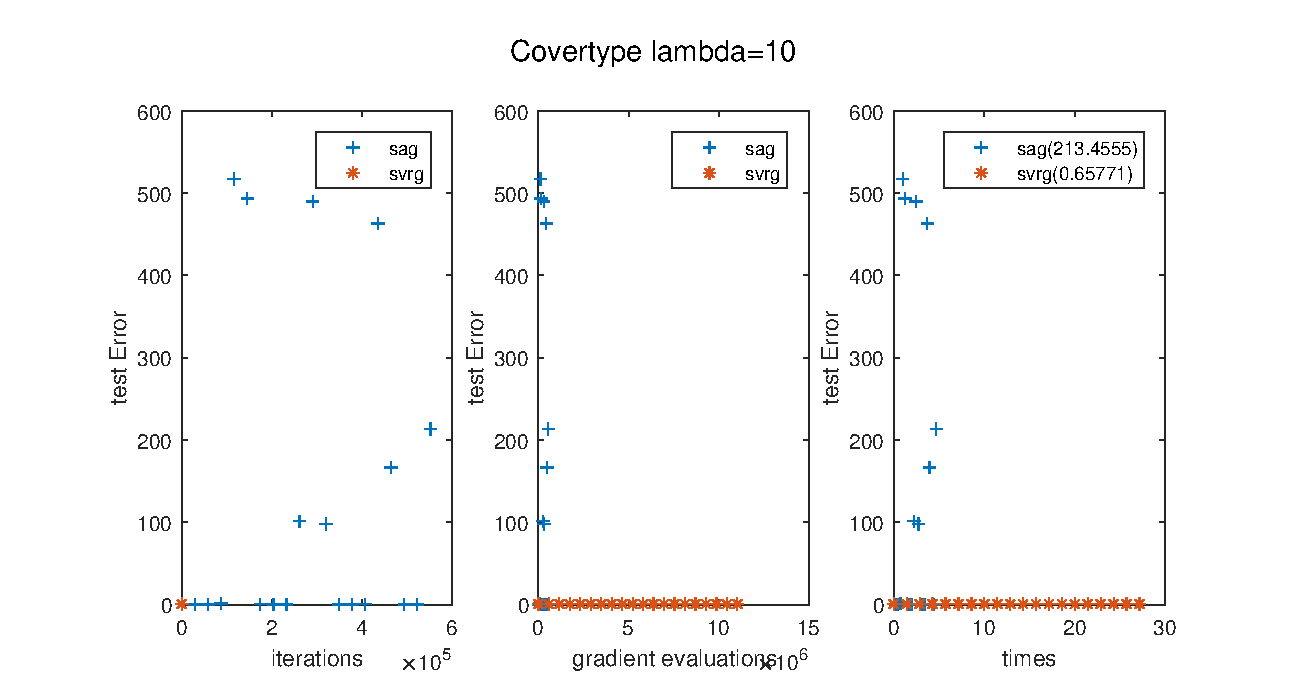
\includegraphics[width=5in]{2-10-a.eps}
\label{fig:2-10-a}
\end{figure}
\begin{figure}[htbp]
\centering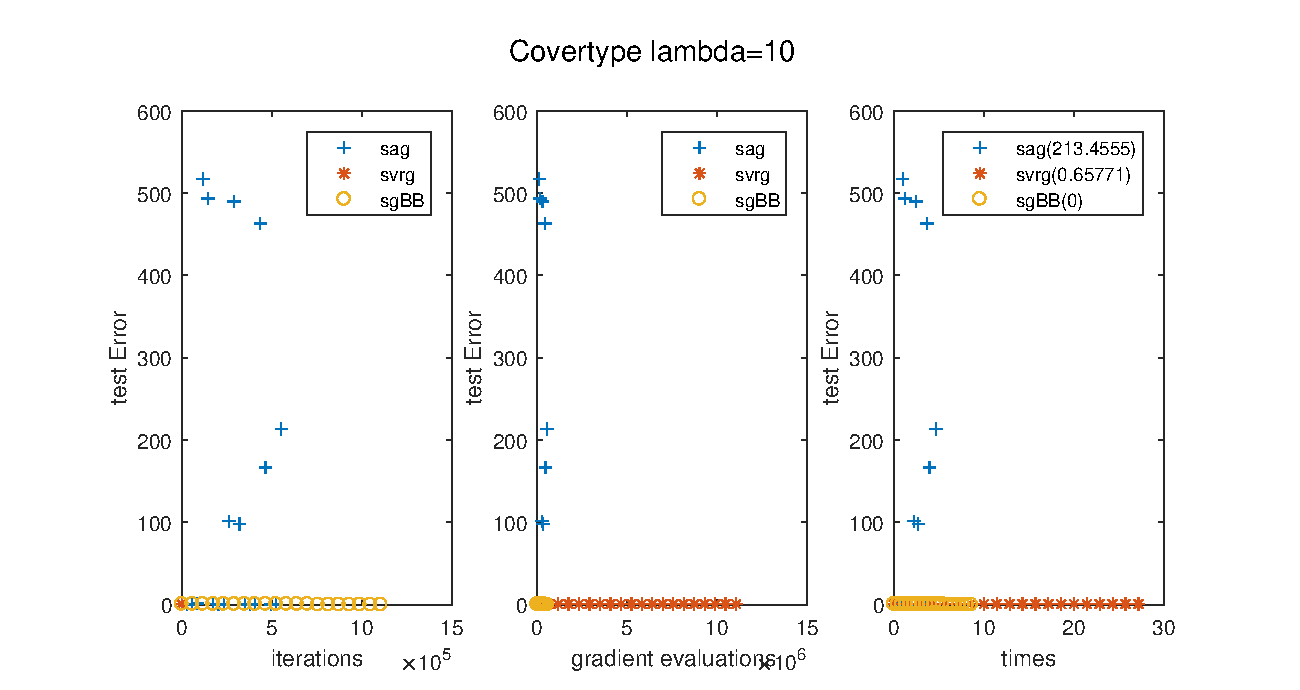
\includegraphics[width=5in]{2-10-b.eps}
\label{fig:2-10-b}
\end{figure}

\begin{figure}[htbp]
\centering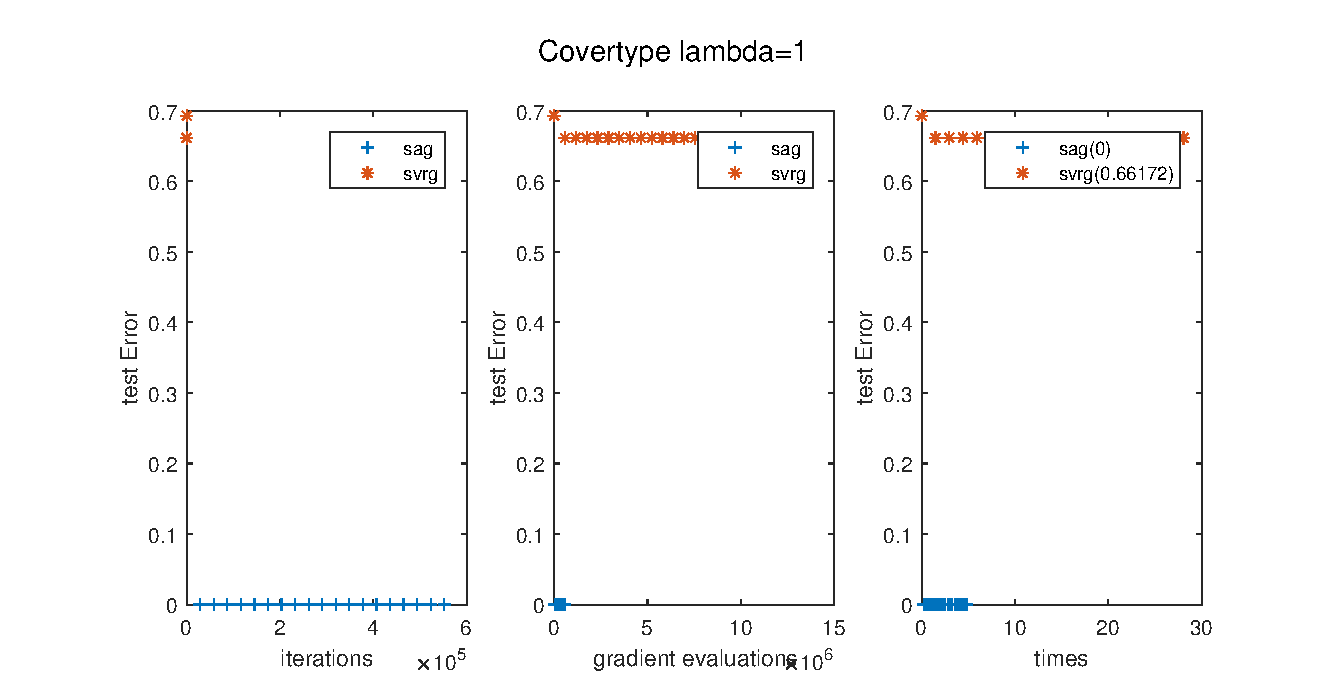
\includegraphics[width=5in]{2-1-a.eps}
\label{fig:2-1-a}
\end{figure}

\begin{figure}[htbp]
\centering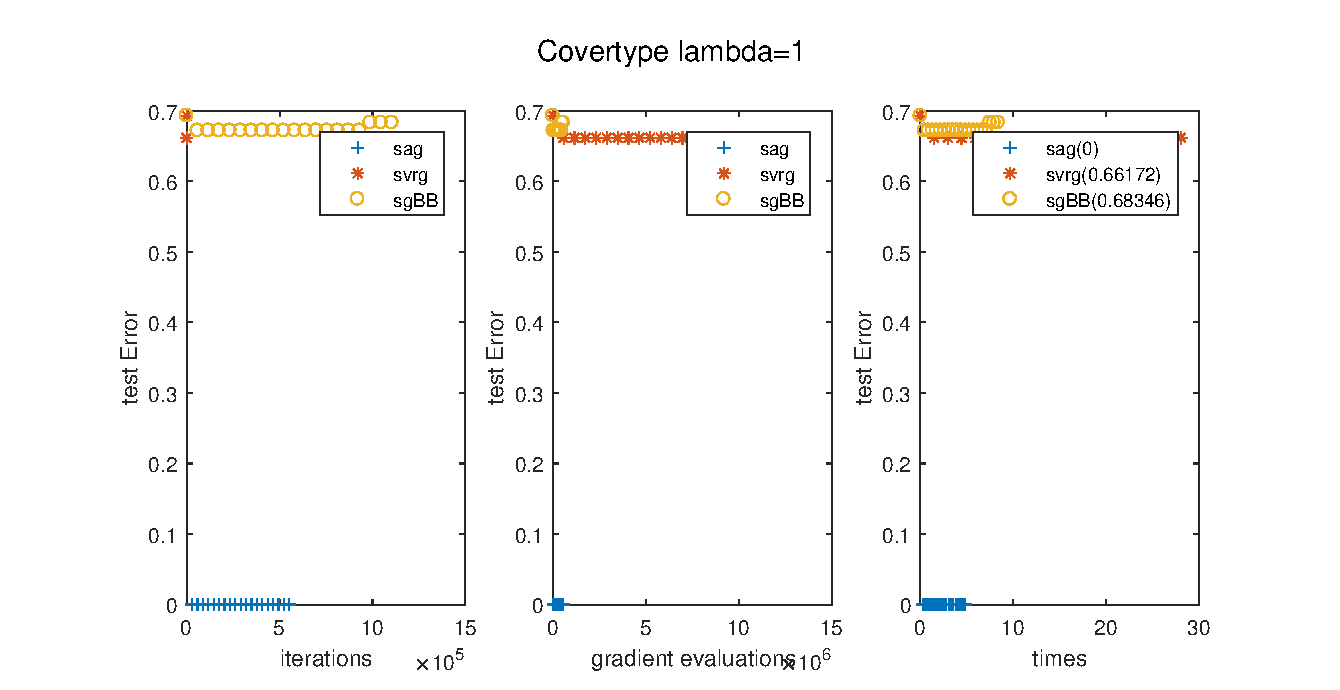
\includegraphics[width=5in]{2-1-b.eps}
\label{fig:2-1-b}
\end{figure}

\begin{figure}[htbp]
\centering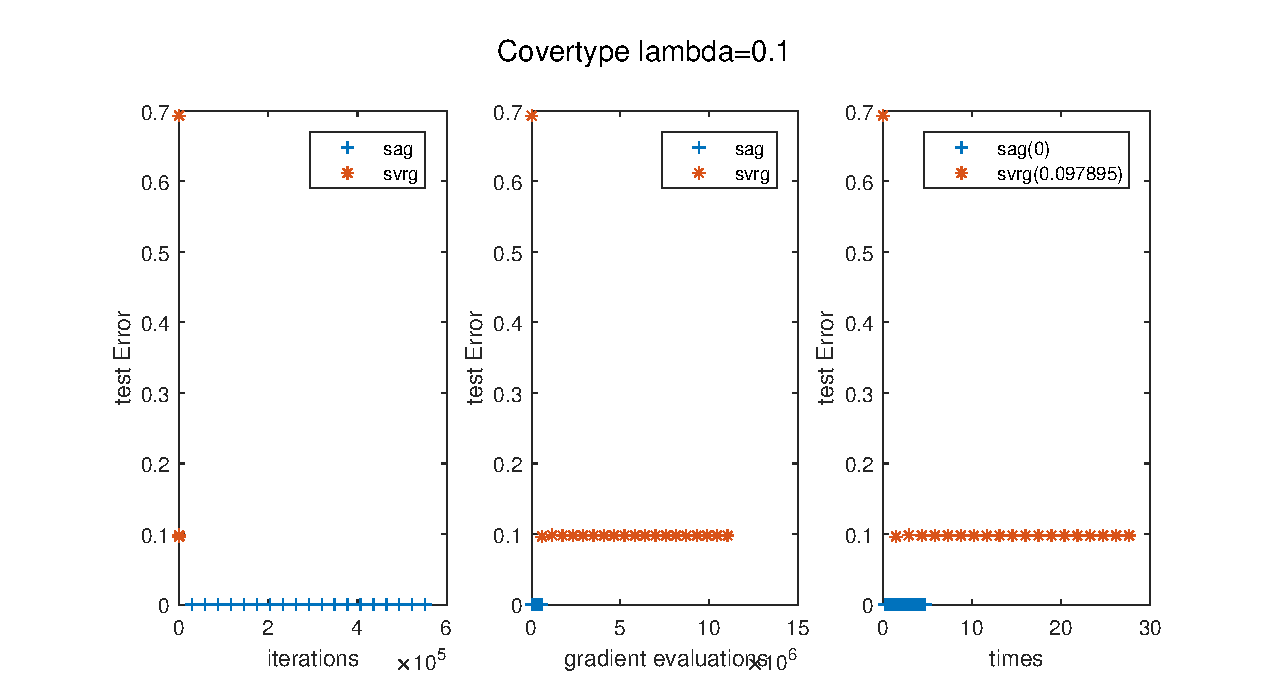
\includegraphics[width=5in]{2-01-a.eps}
\label{fig:2-0.1-a}
\end{figure}

\begin{figure}[htbp]
\centering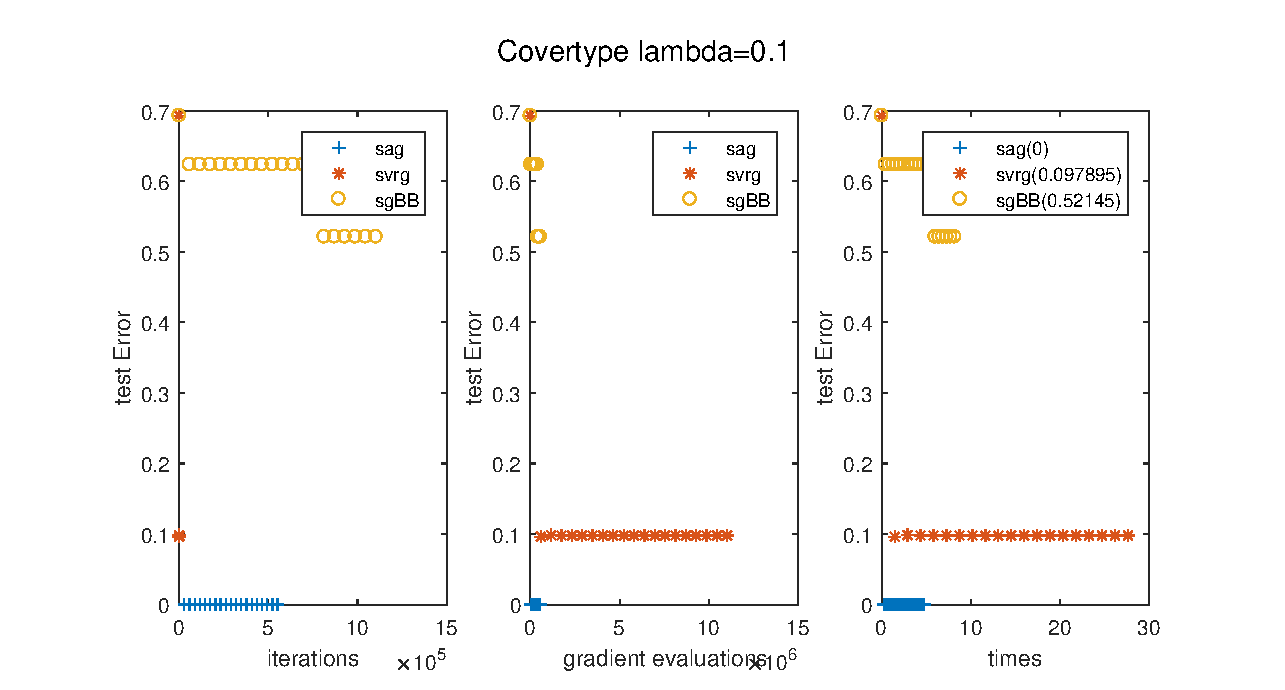
\includegraphics[width=5in]{2-01-b.eps}
\label{fig:2-0.1-b}
\end{figure}
\begin{figure}[htbp]
\centering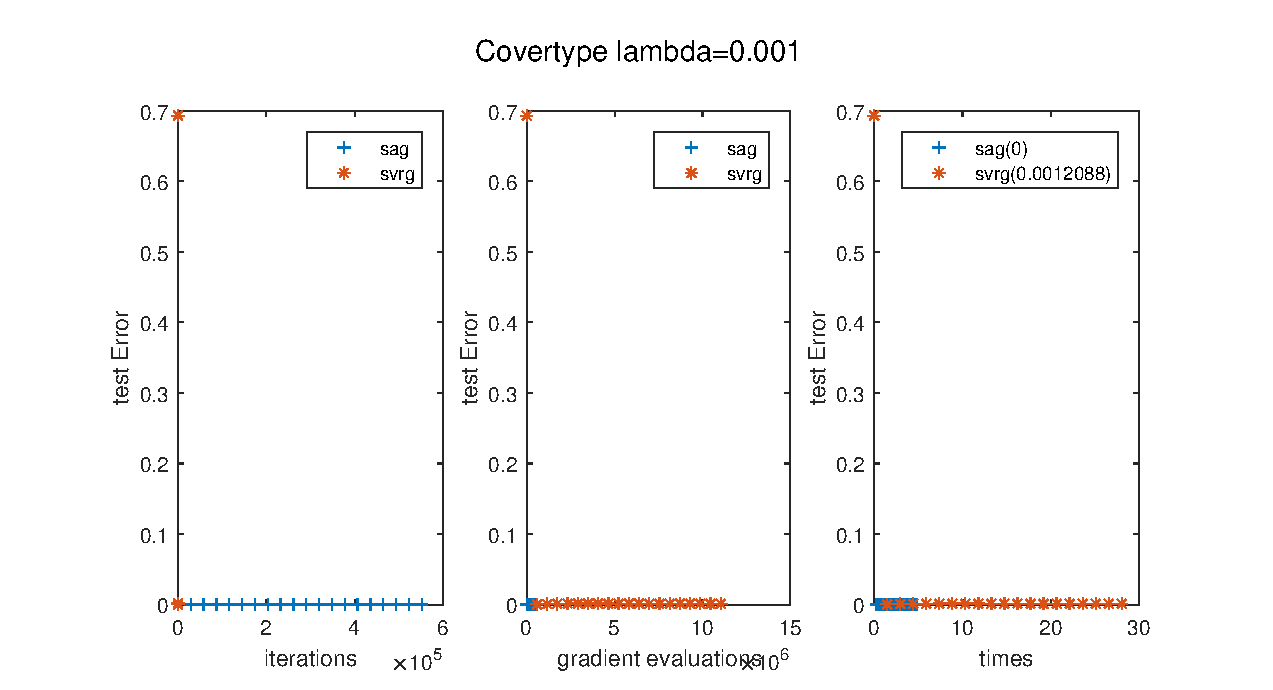
\includegraphics[width=5in]{2-0001-a.eps}
\label{fig:2-0.001-a}
\end{figure}
\begin{figure}[htbp]
\centering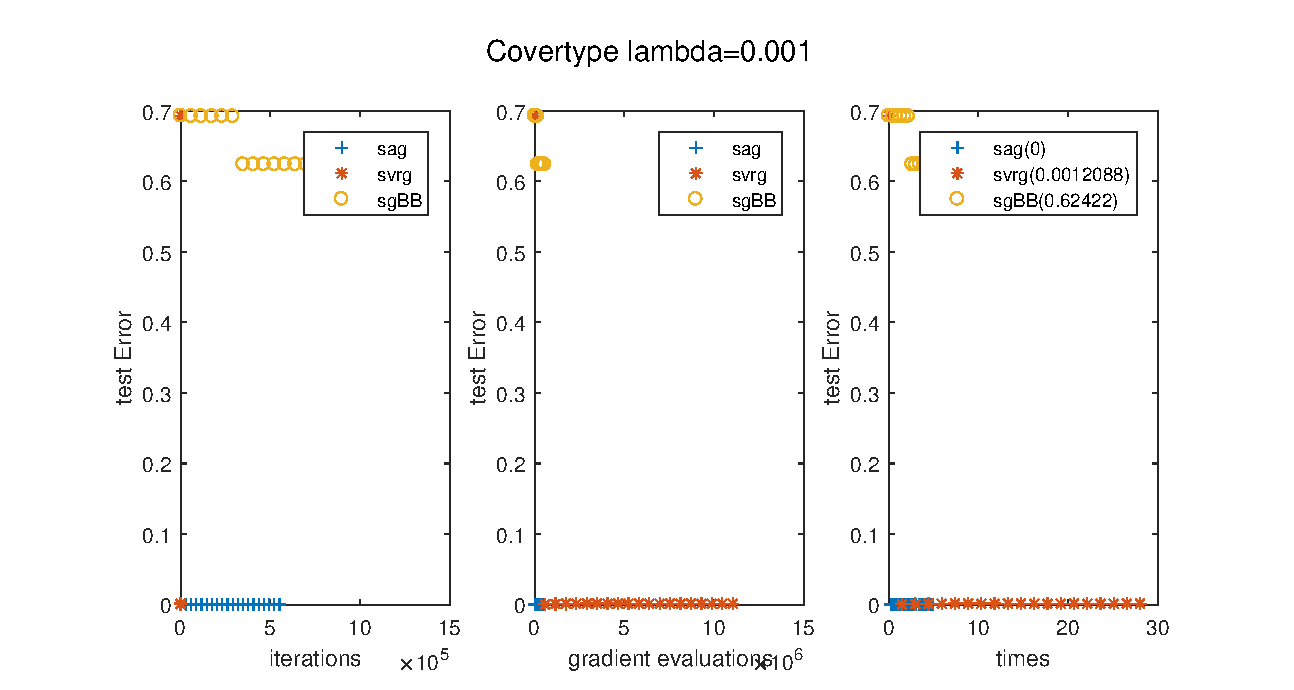
\includegraphics[width=5in]{2-0001-b.eps}
\label{fig:2-0.001-b}
\end{figure}
\begin{figure}[htbp]
\centering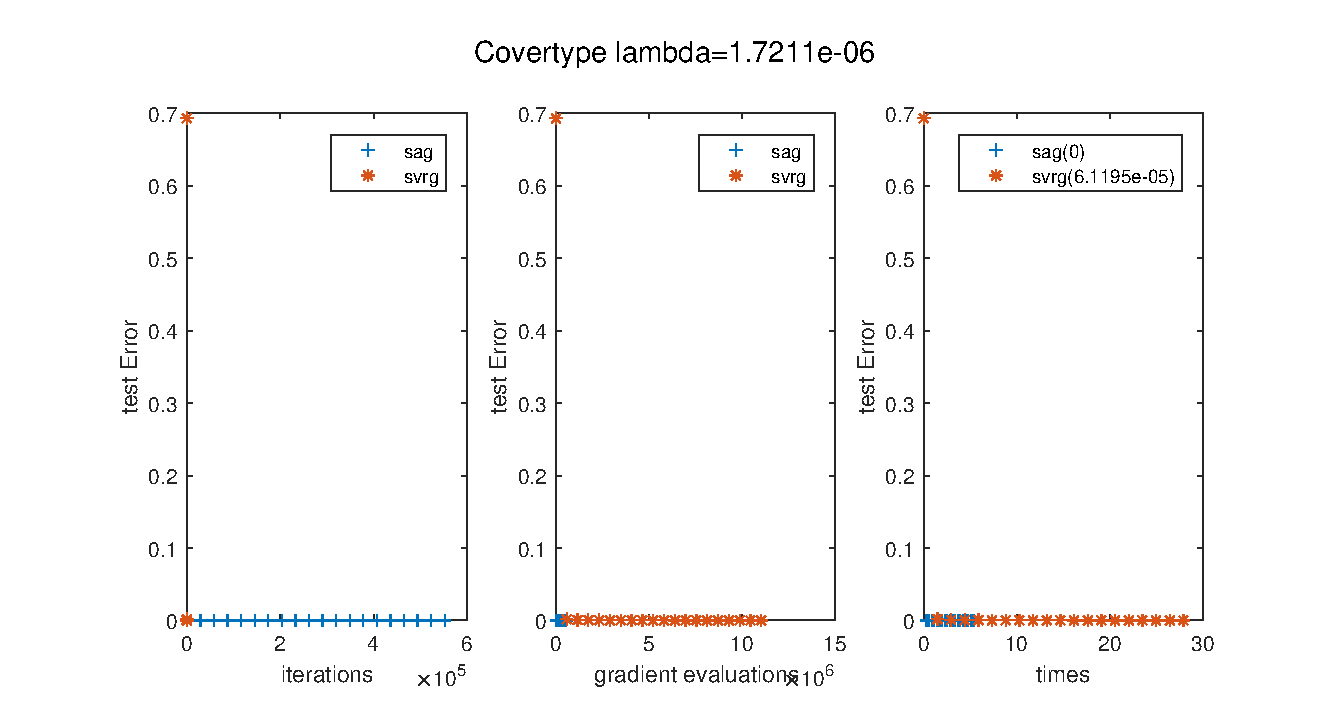
\includegraphics[width=5in]{2-n-a.eps}
\label{fig:2-n-a}
\end{figure}
\begin{figure}[htbp]
\centering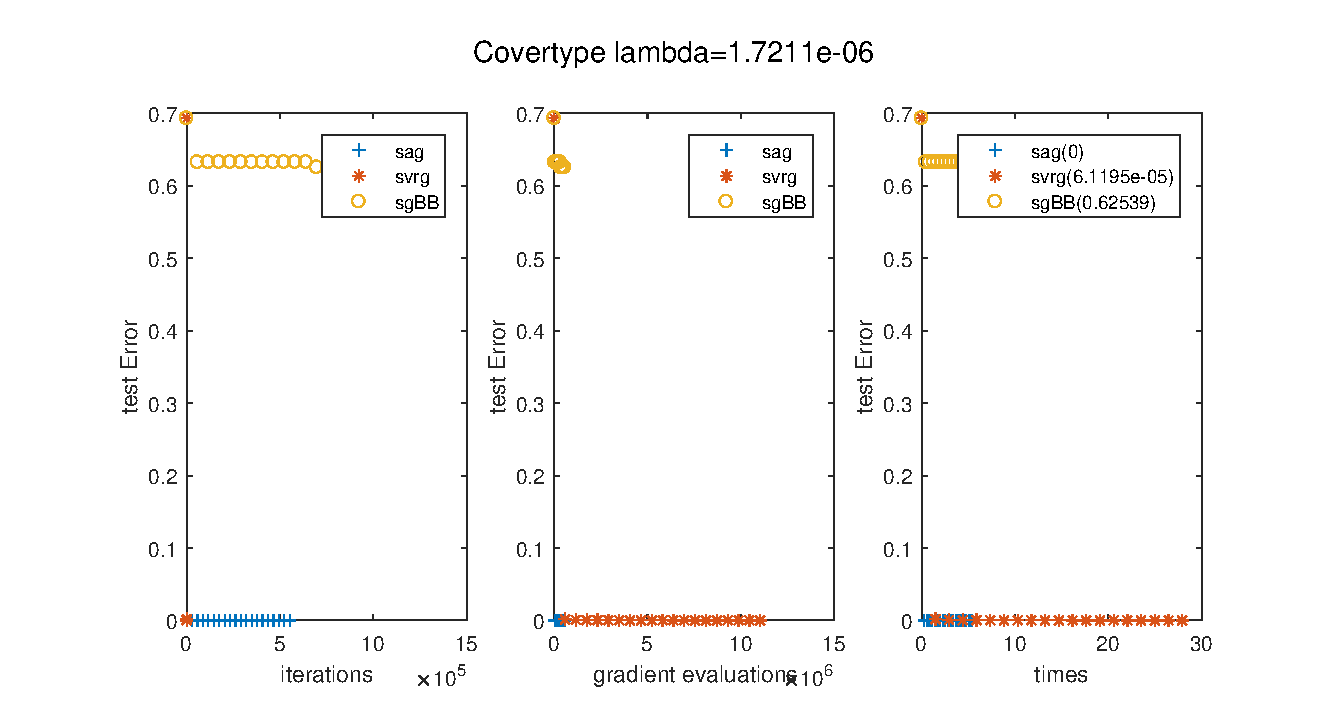
\includegraphics[width=5in]{2-n-b.eps}
\label{fig:2-n-b}
\end{figure}

\begin{figure}[htbp]
\centering\includegraphics[width=5in]{2-n-c.eps}
\caption{}\label{fig:2-n-c}
\end{figure}

\begin{figure}[htbp]
\centering\includegraphics[width=5in]{2-n-sag.eps}
\caption{}\label{fig:2-n-sag}
\end{figure}



\subsection{结果分析}
\begin{itemize}
  \item 对于两个数据集,随着$\lambda$的减小,SVRG得到的ERROR随之减小,直至1/n时,error能接近SAG的结果
  \item 对于$\lambda\geq 0.1$的情况,SVRG虽然ERROR比SAG大,然而往往较为稳定
  \item 对于较大的$\lambda$,SAG的TESTING ERROR有较大的波动
  \item $\lambda$较小时,SAG的结果比SVRG的结果要好
  \item 对于数据集MINIST,如图\ref{fig:1-n-sag}所示,SAG的TESTING ERROR随计算时间单调减小
  \item 对于EXTRA-CREDIT中的BB步长SG方法,仅当$\lambda=10$时有最好的结果,其余的情况下ERROR较大
\end{itemize}
  \end{document} 